\let\negmedspace\undefined
\let\negthickspace\undefined
\documentclass[journal]{IEEEtran}
\usepackage[a5paper, margin=10mm, onecolumn]{geometry}
%\usepackage{lmodern} % Ensure lmodern is loaded for pdflatex
\usepackage{tfrupee} % Include tfrupee package

\setlength{\headheight}{1cm} % Set the height of the header box
\setlength{\headsep}{0mm}     % Set the distance between the header box and the top of the text

\usepackage{gvv-book}
\usepackage{gvv}
\usepackage{cite}
\usepackage{amsmath,amssymb,amsfonts,amsthm}
\usepackage{algorithmic}
\usepackage{graphicx}
\usepackage{textcomp}
\usepackage{xcolor}
\usepackage{txfonts}
\usepackage{listings}
\usepackage{enumitem}
\usepackage{mathtools}
\usepackage{gensymb}
\usepackage{comment}
\usepackage[breaklinks=true]{hyperref}
\usepackage{tkz-euclide} 
\usepackage{listings}
% \usepackage{gvv}                                        
\def\inputGnumericTable{}                                 
\usepackage[latin1]{inputenc}                                
\usepackage{color}                                            
\usepackage{array}                                            
\usepackage{longtable}                                       
\usepackage{calc}                                             
\usepackage{multirow}                                         
\usepackage{hhline}                                           
\usepackage{ifthen}                                           
\usepackage{lscape}
\begin{document}
\bibliographystyle{IEEEtran}
\title{8.4.5}
\author{EE25BTECH11002 - Achat Parth Kalpesh }
{\let\newpage\relax\maketitle}
\renewcommand{\thefigure}{\theenumi}
\renewcommand{\thetable}{\theenumi}
\setlength{\intextsep}{10pt} % Space between text and floats
\numberwithin{equation}{enumi}
\numberwithin{figure}{enumi}
\renewcommand{\thetable}{\theenumi}
\parindent 0px



\textbf{Question:}\\
An ellipse is drawn by taking a diameter of the circle $\brak{x-1}^2+y^2=1$ as its semi minor axis and a diameter of the circle $x^2+\brak{y-2}^2=4$ as semi-major axis. If the centre of the ellipse is at the origin and its axes are the coordinate axes, then the equation of the ellipse is 
\begin{multicols}{2}
\begin{enumerate}
    \item $4x^2+y^2=4$ 
    \item $x^2+4y^2=8$
    \item $4x^2+y^2=8$
    \item $x^2+4y^2=1$
\end{enumerate}
\end{multicols}

\textbf{Solution:}\\
The standard equation of a circle is given as
\begin{align}
    \brak{\vec{x}-\vec{c}}^\top\brak{\vec{x}-\vec{c}} = r^2
\end{align}

Given two circles are
\begin{align}
    \brak{\vec{x}-\vec{c_1}}^\top\brak{\vec{x}-\vec{c_1}} = 1\\
    \brak{\vec{x}-\vec{c_2}}^\top\brak{\vec{x}-\vec{c_2}} = 4
\end{align}

The centers and radii are
\begin{align}
    \vec{c_1} = \myvec{1\\0}, \quad r_1 = 1\\
    \vec{c_2} = \myvec{0\\2}, \quad r_2 = 2
\end{align}

Verifing that the origin lies on both circles:
\begin{align}
    \brak{\vec{0}-\vec{c_1}}^\top\brak{\vec{0}-\vec{c_1}} = 1 = r_1^2\\
    \brak{\vec{0}-\vec{c_2}}^\top\brak{\vec{0}-\vec{c_2}} = 4 = r_2^2
\end{align}

Thus, the diameters of both circles passing through the origin are along the directions
\begin{align}
    \vec{c_1} = \myvec{1\\0} \text{ \brak{\text{along X-axis}}}\\
    \vec{c_2} = \myvec{0\\2} \text{ \brak{\text{along Y-axis}}}
\end{align}

Each circle's diameter length is $2r$. Therefore, the ellipse's 
semi-axes are equal to the respective radii:
\begin{align}
    b = r_1 = 1 \quad \text{\brak{\text{semi-minor axis}}}\\
    a = r_2 = 2 \quad \text{\brak{\text{semi-major axis}}}
\end{align}

The standard equation of an ellipse centered at the origin with coordinate axes as its axes is
\begin{align}
    \vec{x}^\top A \vec{x} = 1
\end{align}
where
\begin{align}
    A = \myvec{\frac{1}{b^2} & 0 \\ 0 & \frac{1}{a^2}}
\end{align}

Substituting $a = 2,\, b = 1$,
\begin{align}
    A = \myvec{1 & 0 \\ 0 & \frac{1}{4}}
\end{align}

Hence,
\begin{align}
    \vec{x}^\top\myvec{1 & 0 \\ 0 & \frac{1}{4}}\vec{x} = 1
\end{align}

Multiplying throughout by $4$ gives
\begin{align}
    \vec{x}^\top\myvec{4 & 0 \\ 0 & 1}\vec{x} = 4
\end{align}

or equivalently,
\begin{align}
    4x^2 + y^2 = 4
\end{align}
\begin{figure}[h!]
    \centering
    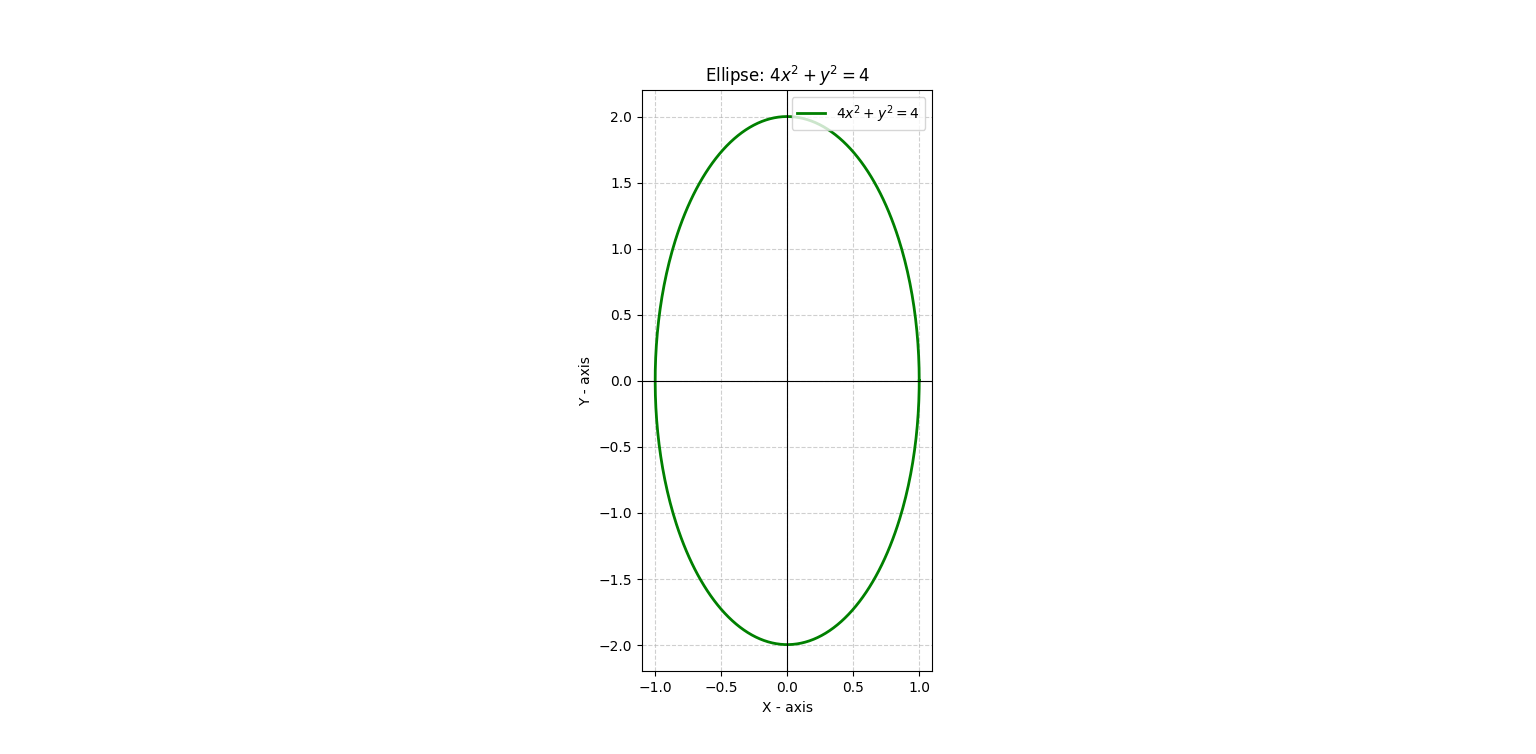
\includegraphics[width=\columnwidth]{figs/figure_py.png}
    \caption{Ellipse}
    \label{fig:fig}
 \end{figure}

\end{document}